\section*{Часть Самарина Артема}

\subsection*{Теоретическая часть}
Моей главной задачей было научиться восстанавливать движения телефона по имеющимся у нас данным – времени, показателям акселерометра и гироскопа.

\subsubsection*{НЕУДАЧНЫЙ СПОСОБ}

Для начала задача решалась самым прямым образом - данные аксселерометра (т.е. ускорение по каждой из осей телефона) дважды интегрировались и таким образом получалаось положение телефона в каждый момент времени, но из=за большой погрешности, двойного интегрирования и помех ничего не вышло – картинка съезжала и вместо допустим нужного квадрата получалась спираль. Изначально, я это списывал на то, что акселерометр учитывает ускорение свободного падения, но это оказалось не так.

\subsubsection*{С ЧЕМ ВООБЩЕ РАБОТАЕМ?}

На вход я получаю массив с 7-ю параметрами: время от начала движения, ускорение по оси X, ускорение по оси Y, ускорение по оси Z, угол поворта по X (Pitch), угол поворота по Y (Roll) и угол поворота по Z (Yaw).

\begin{figure}[H]
    \center{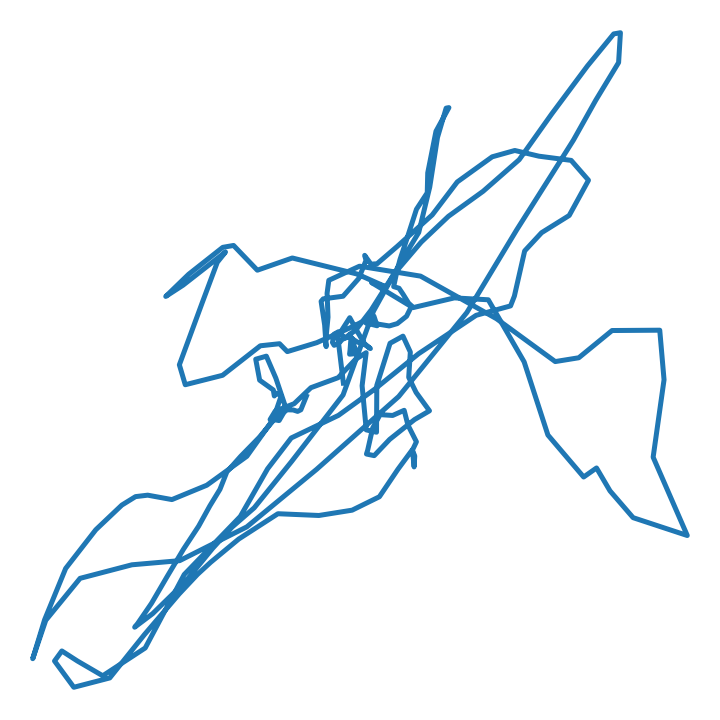
\includegraphics[scale = 0.7]{1.png}}
\end{figure}

\subsubsection*{НОРМАЛИЗАЦИЯ ДАННЫХ}
Для своей задачи я использую 2 фильтра – тот что реализован другим членом моей команды и свой. Мой фильтр сглаживает определенную погрешность. 

\begin{figure}[H]
    \center{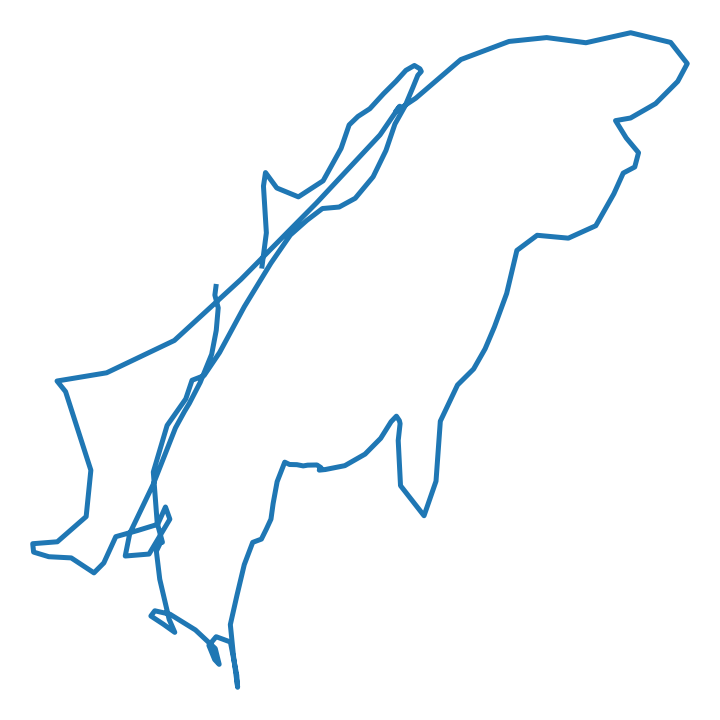
\includegraphics[scale = 0.7]{2.png}}
\end{figure}

А так же из каждого значения акселерометра по каждой оси вычитается среднее по это оси.

\begin{figure}[H]
    \center{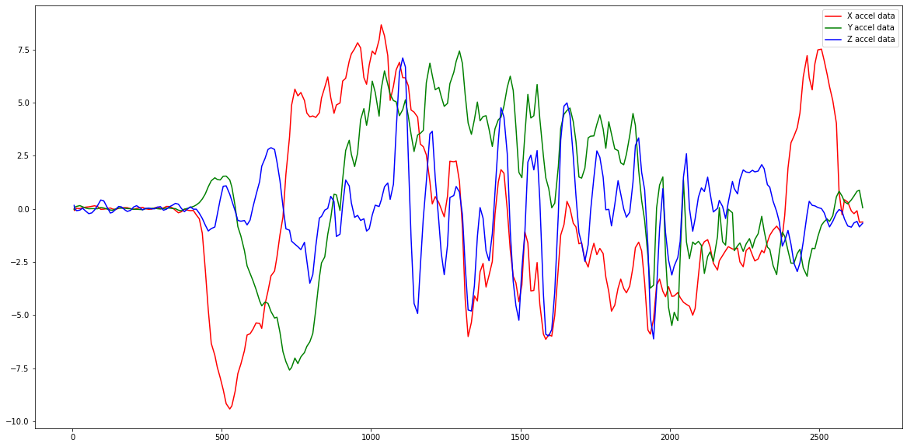
\includegraphics[scale = 0.85]{graph_1.png}}
    \center{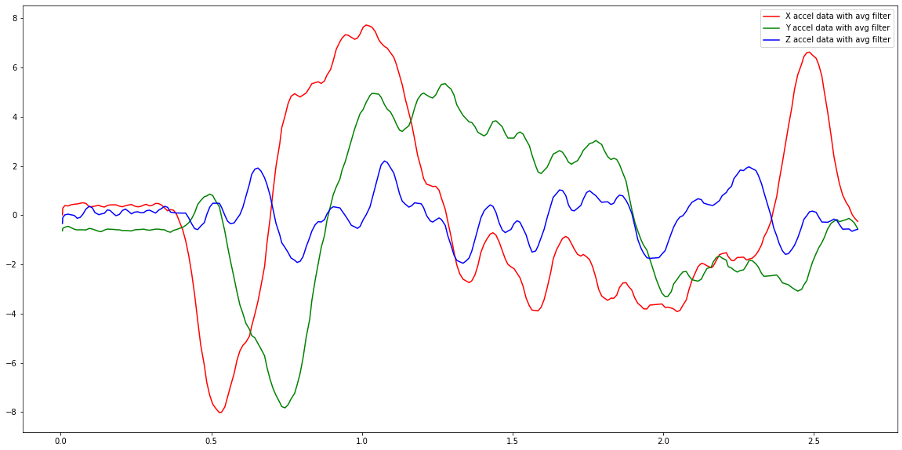
\includegraphics[scale = 0.85]{graph_2.png}}
\end{figure}

\subsubsection*{НАХОЖДЕНИЕ ПОЛОЖЕНИЯ ТЕЛЕФОНА БЕЗ УЧЕТА ДАННЫХ ИЗ ГИРОСКОПА}

После того как данные нормализованы – как уже говорилось ранее – данные акселерометра дважды интегрируются. Если данные акселерометра по X – это вектор А, а время – это вектор T, то положение в каждый момент времени определяется, как $A[i] * (T[i] - T[i-1])$.

\begin{figure}[H]
    \center{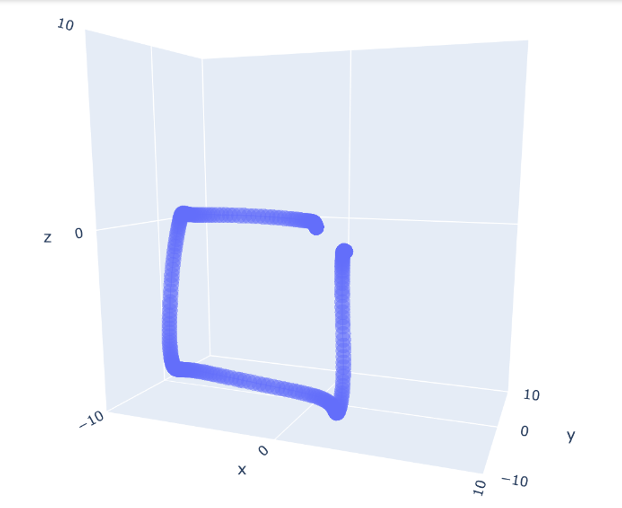
\includegraphics[scale = 0.85]{3d_graph_1.png}}
    \center{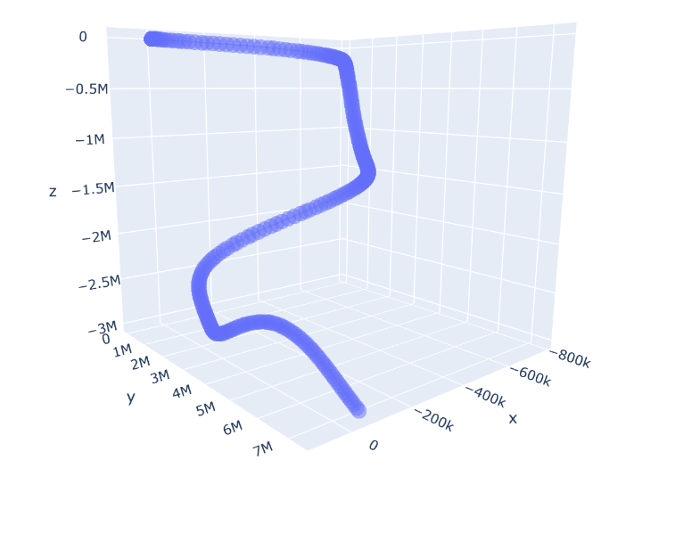
\includegraphics[scale = 0.85]{3d_graph_2.png}}
\end{figure}

\subsubsection*{ПОЧЕМУ И КАК ЭТО РАБОТАЕТ?}

Когда человек рисует жест (а это основной смысл разрабатываемой нами технологии), то он стоит на месте и телефон, как правило, держит в одном положении, просто потому что это удобно – телефоны широкие и как либо менять угол его поворота сложно, если не делать это намеренно. Соответственно, если угол поворота телефона меняется, то хорошее отображение движения телефона не получится.

\subsubsection*{КАК И ЗАЧЕМ УЧИТЫВАТЬ ДАННЫЕ ГИРОСКОПА?}

Данные гироскопа учитываются для того, чтобы компенсировать угол вращения телефона. Если учитывать угол поворота, то можно получить положение телефона относительно земли, а не относительно движения вдоль своих осей.
Для этого берется вектор значений гироскопа в момент времени 0 и умножается на эту матрицу (затехайте пожалуйста matrix [[ cos(z)*cos(y), -sin(z)*cos(x) + cos(z)*sin(x)*sin(y), sin(z)*sin(x)+ cos(x)*cos(z)*sin(y)], [cos(z)*cos(y), cos(z)*cos(x) + sin(x)*sin(y), -cos(z)*sin(x)+ cos(x)*sin(z)*sin(y)], [-sin(y), cos(y)*sin(x), cos(x)*cos(y)]]) и получается угол поворота в следующий момент времени относительно земли. Зная эти углы, мы можем компенсировать движение телефона вокруг своих осей и находить более точное положение телефона в пространстве.

\begin{equation*}
    \begin{pmatrix}
        cos(z)*cos(y) & -sin(z)*cos(x) + cos(z)*sin(x)*sin(y) & sin(z)*sin(x)+ cos(x)*cos(z)*sin(y) \\
        cos(z)*cos(y) & cos(z)*cos(x) + sin(x)*sin(y) & -cos(z)*sin(x)+ cos(x)*sin(z)*sin(y) \\
        -sin(y) & cos(y)*sin(x) & cos(x)*cos(y) \\
    \end{pmatrix}
\end{equation*}
и получается угол поворота в следующий момент времени относительно земли. Зная эти углы, мы можем компенсировать движение телефона вокруг своих осей и находить более точное положение телефона в пространстве.

